% Evidence-limited working manuscript; not submission-ready.
\documentclass[sigconf,review,anonymous]{acmart}
% Keep local syntax checks usable on minimal TeX installations. Overleaf and
% the submission build retain the ACM font and microtype defaults.
\IfFileExists{libertine.sty}{}{\microtypesetup{expansion=false}}
% Figures are TikZ sources generated from the committed records by
% tools/rbq_fig_*.py, so their text is set in the document's own faces and the
% built PDF embeds no font the body does not already carry.
\usepackage{tikz}
\usetikzlibrary{arrows.meta}
% The figures are large multi-panel floats; LaTeX's default placement
% parameters defer them past the bibliography. These are placement limits, not
% typography: no font, measure, leading or float separation is changed.
\setcounter{topnumber}{3}
\setcounter{totalnumber}{4}
\renewcommand{\topfraction}{0.92}
\renewcommand{\textfraction}{0.06}
\renewcommand{\floatpagefraction}{0.72}
\setcopyright{none}
\acmDOI{}
\acmISBN{}
\acmConference[MMSys '27]{18th ACM Multimedia Systems Conference}
  {March 30--April 2, 2027}{Ghent, Belgium}
\acmYear{2027}
\copyrightyear{2027}
\begin{document}

\begin{CCSXML}
<ccs2012>
   <concept>
       <concept_id>10010520.10010570</concept_id>
       <concept_desc>Computer systems organization~Real-time systems</concept_desc>
       <concept_significance>500</concept_significance>
   </concept>
   <concept>
       <concept_id>10010520.10010553.10010562</concept_id>
       <concept_desc>Computer systems organization~Embedded systems</concept_desc>
       <concept_significance>500</concept_significance>
   </concept>
   <concept>
       <concept_id>10010147.10010178.10010224.10010225.10010233</concept_id>
       <concept_desc>Computing methodologies~Vision for robotics</concept_desc>
       <concept_significance>300</concept_significance>
   </concept>
   <concept>
       <concept_id>10011007.10010940.10011003.10011002</concept_id>
       <concept_desc>Software and its engineering~Software performance</concept_desc>
       <concept_significance>300</concept_significance>
   </concept>
</ccs2012>
\end{CCSXML}


% Title history, retained so the change is traceable. The R17/R18 working title
% was "When Near-30 FPS Is Not Enough: Fail-Closed Qualification of
% Multi-Stream Stereo on One Edge NPU", written for a six-camera target. The
% RBQ-only interim revision used "Four Cameras on One Edge NPU: A
% Value-Preserving Repair of Block-Floating-Point Loss and Two Measured
% Shortfalls". Proposed working title for the restored four-camera retarget,
% used below.
\title[Qualifying Four-Camera Stereo on One Edge NPU]{Qualifying Four-Camera Stereo on One Edge NPU: A Passing Operating Point, Its Scaling Limit, and a Value-Preserving Repair of Block-Floating-Point Loss}
\begin{abstract}
A quadruped robot using four 30-Hz stereo cameras for foothold perception requires 120 stereo-pair inferences per second from a single embedded accelerator. We evaluate whether an AMD XDNA2 neural processing unit (NPU) can sustain this workload under an artifact-bound, fail-closed protocol that independently verifies disparity accuracy, NPU-only execution, raw-output integrity, and sustained runtime while disallowing CPU neural fallback.
With a common stereo model and synchronized replay, two deployment organizations passed all frozen criteria in three 600-s trials: a process-isolated two-process layout sustained 120.0 pair-FPS with p99 latency of 24.31 ms, while a single-session joint layout sustained 119.97 pair-FPS with p99 latency of 28.44 ms. Across two 20-scene benchmark sets, the same model achieved lower endpoint error than the device-default stereo method in every scene and seed (\(p_{\mathrm{holm}}=3.81\times10^{-6}\)); no corresponding Bad3 advantage is claimed.
The experiments further show that nominal single-pair latency alone is insufficient to predict multi-camera feasibility. For an 8.08-ms model, all sustained four-stream checks failed with one shared session yet passed with four process-isolated sessions at the same offered load. A joint organization reduced compute cost relative to four separate calls but still produced replaced frames despite approximately 30 FPS per stream. Thus, execution topology and output integrity can determine real-time feasibility even when average throughput appears sufficient.
A separate block-floating-point study showed that channel permutation, which is identical in exact arithmetic and requires neither retraining nor ground-truth selection, recovered 98.0\% of the accuracy loss observed on silicon, although the resulting graph was too slow for the four-stream budget. Physical tests with four stereo cameras likewise sustained 30 FPS per stream without replacement in three 600-s trials, while OAK end-to-end completion latency remained longer than one frame period. These results establish four-stream XDNA2 stereo feasibility under specific deployment organizations while identifying scheduling, numerical representation, and end-to-end freshness as distinct constraints that throughput alone does not capture.

\end{abstract}
\ccsdesc[500]{Computer systems organization~Real-time systems}

\ccsdesc[500]{Computer systems organization~Embedded systems}

\ccsdesc[300]{Computing methodologies~Vision for robotics}

\ccsdesc[300]{Software and its engineering~Software performance}

\keywords{neural stereo, multi-camera systems, edge inference, block floating point, NPU scheduling}
\maketitle

\section{Introduction}


\begin{figure}
    \centering
    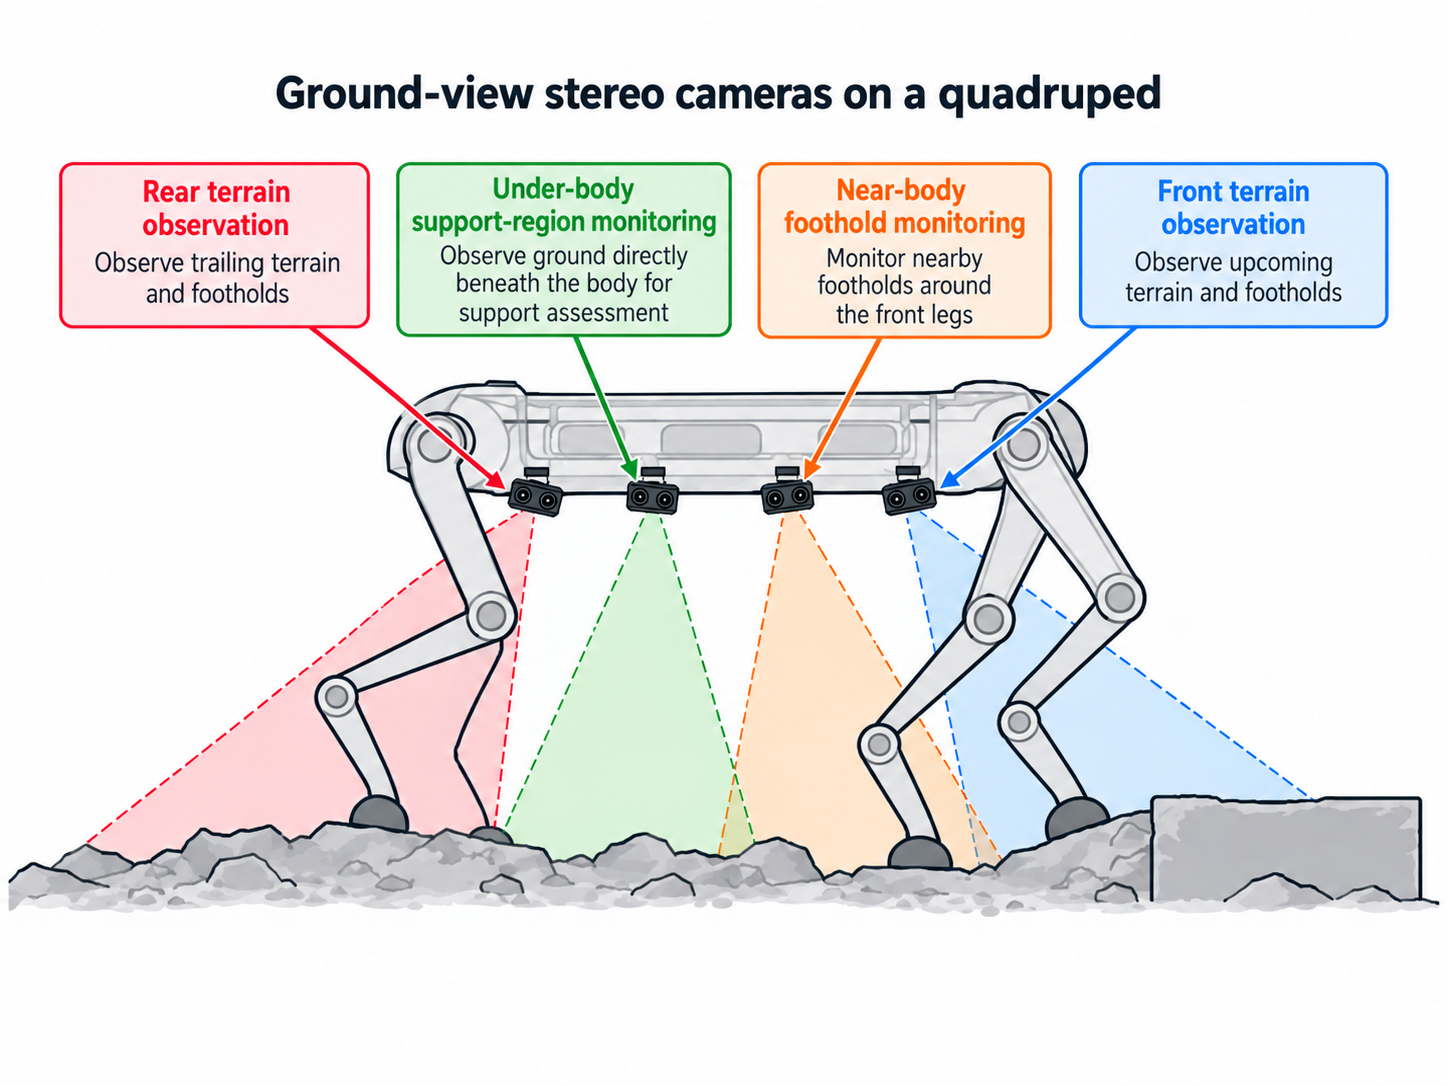
\includegraphics[width=0.7\linewidth]{fig/quad_cam.png}
    \caption{Quadropped robot camera locations and roles}
    \label{fig:QuadCam}
\end{figure}
A quadruped robot carries four stereo cameras beneath its body and computes their disparity maps with their own algorithm as shown in Fig~\ref{fig:QuadCam}. 

However, classical stereo matching methods rely heavily on handcrafted matching costs and fixed optimization rules, making them sensitive to low-texture regions, repetitive patterns, occlusions, illumination changes, and reflective surfaces. Their performance also depends strongly on manually tuned parameters and often degrades when scene characteristics differ from those assumed during algorithm design.

As one of solutions for this, Stereo model based on Artificial Intelligence were suggested. Some stereo model succeed to achieve better performance than the classical stereo model. However, the models are too heavy to run on an edge computer.

A trial in this paper is to make a real-time stereo model for four stereo cameras in quadruped on a neural process unit(NPU).
Each camera must receive its own output at about 30 frames per second, so the accelerator must deliver 120 stereo pairs per second with no neural operation on the host.

%The robot geometry sets the distances that matter. Its dimensional drawing and vendor simulation configuration place the body reference 0.48\textasciitilde0.50 m above level ground, the four optical centres at about 45\textasciitilde48 cm, and its specification states a 25c\textasciitildem maximum step height. A horizontal surface at that height crosses the central optical axes at 20\textasciitilde27 cm and the field corners at about 17 cm, so the application emphasizes a near range of roughly 0.15\textasciitilde0.5 m. \emph{We measured no accuracy in that range}: every accuracy result here comes from benchmark scenes whose disparities do not exercise it, so the geometry motivates the stream count and the response budget, not near-range performance.

The study runs two tracks on one accelerator. A \emph{runtime-control} track holds learned weights fixed across sequential, process-isolated logical and joint-input organizations and asks which satisfies the frozen gates at which stream count; a \emph{specialization} track trains a separate model per organization. Accuracy from one model may not be combined with another model's runtime, and logical processes and compiled subgraphs may share one physical accelerator region, so physical partitioning is an optional extension. A second campaign on the same board characterizes the vendor's block floating-point path with a different model and criterion. The decision rule is speed first: a candidate sustaining the four-stream rate proceeds even where its accuracy does not beat the device-default comparator on every comparison. Accuracy is still measured on the accelerator and reported in full; no floor is assumed because none was set.

This work contributes the following.
\begin{itemize}
\item A four-stream operating point under one frozen protocol: with the common control, a process-isolated pair organization and the joint organization meet every gate across three 600-s repetitions rate or replacement gates on the same weights, under one admission protocol keeping timing failures, integrity failures and incomplete measurements distinct.
\item A two-artifact, three-organization comparison at one offered load in which the organization, not the accelerator's speed, decides the sustained verdict, one artifact failing every sustained check under a single session and passing every one under four process-isolated sessions---and passing them again when fed by four physical cameras of two models, where the capture path rather than the accelerator dominates the response.
\item A frozen negative quantization result: all eight specialized candidates passed the development accuracy gate in full precision, none of their fixed 8-bit exports did, and a recovery that did pass stopped at its first raw-output check on the board.
\item A value-preserving repair for block floating-point deployment loss, measured on silicon against a random-permutation control, with the comparator miss it cannot repair and two failed geometric repairs.
\end{itemize}

\section{Related Work}
Vision stereo model is long-standing: RAFT-Stereo is recurrent~\cite{raftstereo}, FoundationStereo~\cite{foundationstereo} and its real-time variant~\cite{fastfoundationstereo} target zero-shot generalization, and MobileStereoNet reduces parameters and operations with mobile blocks~\cite{shamsafar2022mobilestereonet}; on edge hardware the matcher has been compressed by distillation then pruning~\cite{rbq_pan2024distillprune} and by residual and attention blocks~\cite{rbq_liang2026rcaenet}. The graphs here belong to the reduced-resolution cost-volume family with two-dimensional aggregation, as in HITNet's tile hypotheses~\cite{rbq_tankovich2021hitnet} and LightStereo's channel-boosted three-dimensional volume~\cite{rbq_guo2025lightstereo}. Each reports accuracy and frame rate for a single pair without qualifying a multi-stream deployment against a reference. This study claims no new architecture; it asks whether trained exports survive multi-stream, exact-output, placement and timing qualification. Multi-camera edge systems exploit content overlap: CrossRoI removes redundant regions across overlapping views~\cite{guo2021crossroi} and MOSAIC packs selected regions from concurrent streams into one inference canvas~\cite{gokarn2023mosaic}; our joint arrangement amortizes an invocation but preserves complete, independent stereo pairs and makes no content-selection claim. For inference systems, predictable execution~\cite{clockwork}, fine-grained GPU sharing~\cite{salus}, batched video-DNN scheduling~\cite{nexus}, preemptive time-multiplexing~\cite{prema}, colocation on a fissionable array~\cite{planaria} and, on device, multi-DNN coordination~\cite{rbq_jeong2022band} and preemption on mobile edge GPUs~\cite{rbq_han2024pantheon} motivate separating service time, queueing, batching and tail response, but assume controls this installation does not expose: ours uses ordinary processes and sessions, so what remains is the count of sessions holding the device. Reliability studies trace injected faults through accelerators~\cite{li2017dnnresilience}, protect inference from bit flips~\cite{zheng2025save} or restrict ranges~\cite{rbq_chen2021ranger}, and field reports describe processors computing incorrect results without raising any error, visible only against a reference~\cite{rbq_hochschild2021cores}. They motivate the end-to-end output validation used here as an admission condition rather than a statistic.

Narrow numerical formats for inference increasingly take the form of block floating point, a group of adjacent elements sharing one exponent, each keeping a sign and a short mantissa. Microsoft Floating Point introduced it at production scale~\cite{rbq_rouhani2020msfp}; it was standardized as the Microscaling formats~\cite{rbq_rouhani2023microscaling} and by the Open Compute Project~\cite{rbq_ocp2023mx}, and architectural studies examine such blocks for training~\cite{rbq_zhang2022fast} and serving~\cite{rbq_lee2025mxplus}. The accelerator here exposes a format of the same family~\cite{rbq_amdquarkbfp16}, and because its block boundaries fall along a convolution's input-channel axis, the assignment of channels to blocks is a property of the graph rather than of the format: this work treats that assignment as the quantity to be chosen.

A second thread makes quantization groups more homogeneous by reordering the tensor rather than rewriting it: clustering activation channels by observed range~\cite{rbq_yuan2023rptq}, sorting by a joint statistic of activations and weights~\cite{rbq_cheng2026permuquant}, pairing an outlier channel with low-magnitude companions~\cite{rbq_yao2026ocgquant}, and, outside quantization, permuting a weight matrix so that different weights survive an N:M pruning pattern~\cite{rbq_pool2021permutations}. These differ from transforms that repair quantization by changing values---cross-layer equalization~\cite{rbq_nagel2019dfq}, range migration into the weights~\cite{rbq_xiao2023smoothquant}, activation-aware scaling~\cite{rbq_lin2024awq}, Hadamard rotation~\cite{rbq_ashkboos2024quarot}---and from post-calibration parameter repairs, adaptive rounding~\cite{rbq_nagel2020adaround} and bias correction~\cite{rbq_nagel2019dfq}. This work belongs to the reordering side and differs on the first point only: it regroups channels without altering any stored value, so the floating-point graph remains an identity of the original. It is not distinguished by dispensing with labels, since those methods are calibration-only as well and the permutation was itself selected on thirty-two fixed training frames. Studies of deployment on commercial accelerators repeatedly find that vendor abstractions do not predict real graphs, whether through the software stack~\cite{rbq_hadidi2019characterizing}, operator fusion the operator list hides~\cite{rbq_zhang2021nnmeter}, the compiler's mapping to the memory hierarchy~\cite{rbq_seshadri2022edgetpu} or undisclosed microarchitecture~\cite{rbq_park2026lens}; the observations here are of that kind.

\section{Problem Formulation}
\label{sec:prob}
Two rates are distinguished throughout. \emph{Pair throughput} is the number of disparity maps per second, \emph{invocation throughput} the number of accelerator calls per second. Four cameras at 30 FPS require 120 pair-FPS. A pair arrangement computing one pair per call needs 120 calls per second, a mean service time of at most 8.333 ms; a joint arrangement consuming all four pairs in one call needs 30 calls per second, or at most 33.333 ms. These budgets precede queueing and host work.

Live-input response is measured from capture to completion of disparity decoding. In camera-free replay the pair harness measures from each frame's scheduled arrival, including dispatch lag, the joint harness from release of a synchronized bundle, including its assembly; both exclude capture, transport and camera preprocessing, and their p99 pools completed stream outputs in a window. For $n$ streams the replay gate requires exactly $n$ streams, at least 29.5 FPS each and $29.5n$ aggregate pair-FPS, a minimum/maximum rate ratio of at least 0.98, replacement at most 2\%, p99 at most 40 ms, no raw mismatch and no CPU neural node. The frozen six-stream form of the aggregate criterion was 177 pair-FPS; the same rule at four streams gives 118 pair-FPS, a proportional restatement and not a new measurement. These finite-window criteria are not the strict 30.0-FPS target, which the policy states as four streams and three 600-s repetitions with every stream reaching 30.0 FPS after rounding half up to one decimal. The joint organization additionally incurs an input wait: four uniformly staggered 30-FPS streams make the earliest frame of a same-cycle batch wait 25.0 ms, leaving at most 15.0 ms of joint service under a 40-ms pooled response requirement---a conditional budget, not a limit for mixed-cycle or partial batches. The two campaigns are judged under non-nested replacement rules: this replay gate allows 2\% replacement and requires p99 at most 40 ms, while the second campaign's preregistrations admit no replaced frame and state no response criterion. Exchanging them would change two cells of Table~\ref{tab:sustained}---S5's joint windows would pass this gate and its sequential windows would fail it---while S11's joint windows fail under either rule.

The outcome is definded as fail-closed. \emph{Performance-negative} means recorded outputs are intact but a timing or rate gate fails; \emph{integrity-negative} means a bound-oracle raw comparison fails; \emph{incomplete} means a required measurement is missing; \emph{unknown} means a conditional gate was never evaluated. Missing evidence is never converted into a result: a configuration whose raw output differs from its bound literal oracle is excluded even if its rate meets the target, and if none passes, none is reported suitable rather than substituting CPU inference.

\section{System and Model}

\begin{figure}[t]
\centering
% Generated by tools/rbq_fig_*.py from committed records. Do not edit by
% hand: regenerate instead, so the figure and its manifest entry stay in
% step. Records read are listed in
% experiments/mmsys2027_rbq_retarget_20260914/paper_figures_20260915/FIGURES_R1.json.
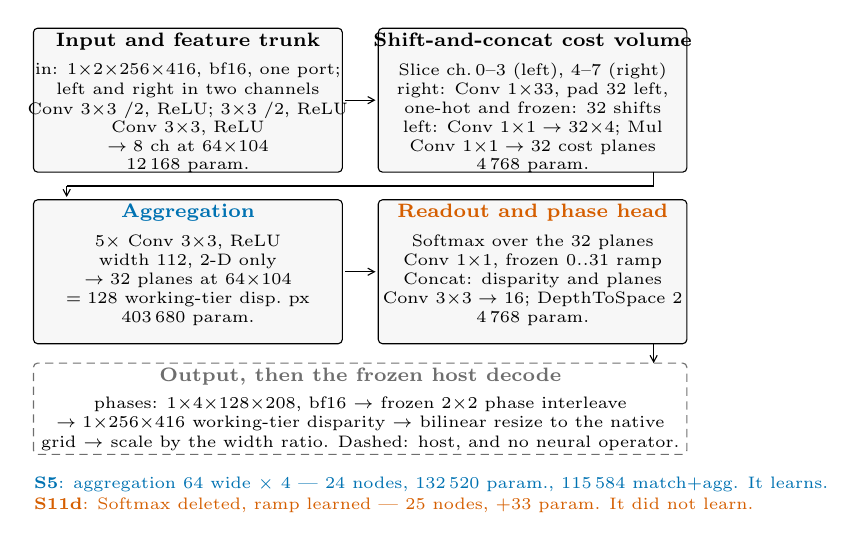
\begin{tikzpicture}[x=1pt,y=1pt,line width=0.4pt]
\definecolor{figblue}{RGB}{0,114,178}
\definecolor{figverm}{RGB}{213,94,0}
\definecolor{figgrey}{RGB}{110,110,110}
\providecommand{\fsix}{\fontsize{6}{7}\selectfont}
\tikzset{stage/.style={draw=black,rounded corners=1.5pt,fill=black!3},host/.style={draw=figgrey,densely dashed,rounded corners=1.5pt},flow/.style={-{Straight Barb[length=2.4pt,width=2.6pt]},draw=black}}
\draw[stage] (0.0,124.0) rectangle (111.6,176.0);
\node[anchor=north,inner sep=0pt,font=\scriptsize\bfseries] at (55.8,174.5) {Input and feature trunk};
\node[anchor=north,inner sep=0pt,font=\fsix] at (55.8,163.5) {in: $1{\times}2{\times}256{\times}416$, bf16, one port;};
\node[anchor=north,inner sep=0pt,font=\fsix] at (55.8,156.6) {left and right in two channels};
\node[anchor=north,inner sep=0pt,font=\fsix] at (55.8,149.7) {Conv $3{\times}3$ /2, ReLU; $3{\times}3$ /2, ReLU};
\node[anchor=north,inner sep=0pt,font=\fsix] at (55.8,142.8) {Conv $3{\times}3$, ReLU};
\node[anchor=north,inner sep=0pt,font=\fsix] at (55.8,135.9) {$\to 8$ ch at $64{\times}104$};
\node[anchor=north,inner sep=0pt,font=\fsix] at (55.8,129.0) {12\,168 param.};
\draw[stage] (124.6,124.0) rectangle (236.1,176.0);
\node[anchor=north,inner sep=0pt,font=\scriptsize\bfseries] at (180.4,174.5) {Shift-and-concat cost volume};
\node[anchor=north,inner sep=0pt,font=\fsix] at (180.4,163.5) {Slice ch.\,0--3 (left), 4--7 (right)};
\node[anchor=north,inner sep=0pt,font=\fsix] at (180.4,156.6) {right: Conv $1{\times}33$, pad 32 left,};
\node[anchor=north,inner sep=0pt,font=\fsix] at (180.4,149.7) {one-hot and frozen: 32 shifts};
\node[anchor=north,inner sep=0pt,font=\fsix] at (180.4,142.8) {left: Conv $1{\times}1 \to 32{\times}4$; Mul};
\node[anchor=north,inner sep=0pt,font=\fsix] at (180.4,135.9) {Conv $1{\times}1 \to 32$ cost planes};
\node[anchor=north,inner sep=0pt,font=\fsix] at (180.4,129.0) {4\,768 param.};
\draw[stage] (0.0,62.0) rectangle (111.6,114.0);
\node[anchor=north,inner sep=0pt,font=\scriptsize\bfseries,text=figblue] at (55.8,112.5) {Aggregation};
\node[anchor=north,inner sep=0pt,font=\fsix] at (55.8,101.5) {5$\times$ Conv $3{\times}3$, ReLU};
\node[anchor=north,inner sep=0pt,font=\fsix] at (55.8,94.6) {width 112, 2-D only};
\node[anchor=north,inner sep=0pt,font=\fsix] at (55.8,87.7) {$\to 32$ planes at $64{\times}104$};
\node[anchor=north,inner sep=0pt,font=\fsix] at (55.8,80.8) {$=128$ working-tier disp.\ px};
\node[anchor=north,inner sep=0pt,font=\fsix] at (55.8,73.9) {403\,680 param.};
\draw[stage] (124.6,62.0) rectangle (236.1,114.0);
\node[anchor=north,inner sep=0pt,font=\scriptsize\bfseries,text=figverm] at (180.4,112.5) {Readout and phase head};
\node[anchor=north,inner sep=0pt,font=\fsix] at (180.4,101.5) {Softmax over the 32 planes};
\node[anchor=north,inner sep=0pt,font=\fsix] at (180.4,94.6) {Conv $1{\times}1$, frozen $0..31$ ramp};
\node[anchor=north,inner sep=0pt,font=\fsix] at (180.4,87.7) {Concat: disparity and planes};
\node[anchor=north,inner sep=0pt,font=\fsix] at (180.4,80.8) {Conv $3{\times}3 \to 16$; DepthToSpace 2};
\node[anchor=north,inner sep=0pt,font=\fsix] at (180.4,73.9) {4\,768 param.};
\draw[host] (0.0,22.0) rectangle (236.1,55.0);
\node[anchor=north,inner sep=0pt,font=\scriptsize\bfseries,text=figgrey] at (118.1,53.5) {Output, then the frozen host decode};
\node[anchor=north,inner sep=0pt,font=\fsix] at (118.1,43.0) {phases: $1{\times}4{\times}128{\times}208$, bf16 $\to$ frozen $2{\times}2$ phase interleave};
\node[anchor=north,inner sep=0pt,font=\fsix] at (118.1,36.0) {$\to 1{\times}256{\times}416$ working-tier disparity $\to$ bilinear resize to the native};
\node[anchor=north,inner sep=0pt,font=\fsix] at (118.1,29.0) {grid $\to$ scale by the width ratio. Dashed: host, and no neural operator.};
\draw[flow] (112.6,150.0) -- (123.6,150.0);
\draw[flow] (112.6,88.0) -- (123.6,88.0);
\draw[draw=black] (224.1,124.0) -- (224.1,119.0) -- (12.0,119.0);
\draw[flow] (12.0,119.0) -- (12.0,115.0);
\draw[flow] (224.1,62.0) -- (224.1,55.0);
\node[anchor=north west,inner sep=0pt,font=\fsix,text=figblue] at (0.0,14.0) {\textbf{S5}: aggregation 64 wide $\times$ 4 --- 24 nodes, 132\,520 param., 115\,584 match$+$agg. It learns.};
\node[anchor=north west,inner sep=0pt,font=\fsix,text=figverm] at (0.0,6.5) {\textbf{S11d}: Softmax deleted, ramp learned --- 25 nodes, $+33$ param. It did not learn.};
\end{tikzpicture}

\caption{The deployed speed-line graph, read node by node from the exported ONNX file of the trained S11 artifact and cross-checked against the screen's recorded geometry: node count, operator histogram, boundary shapes and the four-way parameter split agree exactly for all three variants. The cost volume is a shift and concatenation realized as one convolution with a frozen one-hot $1\times33$ kernel and a left-edge pad, placing 32 disparity planes at the quarter grid. Variants differ only where marked.}%
\label{fig:arch}
\end{figure}

\subsection{Network structure and input--output definitions}
The common runtime-control network, denoted HWGT128, receives rectified grayscale images from the left and right cameras, each of dimensions $1\times1\times256\times416$. Convolutional features form a matching volume indexed by disparity, then aggregation, a learned coupled moment projector and phase-residual refinement. It uses a width multiplier of 1.5 and a two-layer moment projector with 256 channels, and its output has seven channels at $128\times208$: coarse disparity terms, one auxiliary channel and four phase residuals as shown in Fig.~\ref{fig:arch}.

Its inputs use UINT8 with a scale of $1/32$ and a zero point of 114; the output scale and zero point are $1/32$ and 42, and the seven channel multipliers are $(4,4,16,4,4,4,4)$. We use \emph{XINT8} for a fixed static deployment artifact with UNIT8 activations and signed 8-bit weights, scored with the frozen decoder; promoting one also requires every raw replay output to match the frozen CPU oracle bit for bit. Decoding adds and upsamples the first two channels and rearranges the last four into a $2\times2$ residual pattern added to the result, separating cameras before resizing; it is timed and runs no neural layer on the CPU. The specialization track keeps the same input tier, disparity units, output shape and decoder but trains a separate model per execution family: S6 uses hidden widths of 128, 96 and 64 channels, L6 256, 192 and 128, and J6 128 and 96. Each of the eight seed-0 candidates follows a 32-epoch full-precision trajectory and, after the exposed development gate, a fixed 64-epoch quantization-aware one whose terminal epochs alone are eligible. For HWGT128 hardware execution, odd scalar activation zero points were advanced to the next even value, the maximum unsigned value handled separately, and an identity depthwise requantization inserted before a nearest-neighbour resize; that adjustment changes the model and was separately evaluated.

\subsection{Runtime operation and validation}
Selecting the accelerator's execution provider does not by itself ensure full-model execution there~\cite{ortapi,amddeploy}, so each session disables host-provider and Python fallback and inspects compiled contexts first; offline host runs supply references, not measured execution. The capture process retains one pending frame, frames replaced by newer arrivals count towards the replacement rate, and each failure saves inputs, raw outputs, input--output definitions and model hashes together, so a later correct replay does not invalidate a recorded failure.

\section{Execution Organizations}
\label{sec:fam}
Three organizations are admitted and one suffices. In \textbf{T1}, one session uses the full accelerator array and a round-robin scheduler takes the latest pair from each non-empty camera slot, one pair per call, without waiting for all cameras; submission and decoding still require margin below the 8.333-ms single-pair limit. In \textbf{T2L}, camera groups go to separate processes, each owning one session; $k\times m$ denotes $k$ processes serving $m$ cameras each, the four-stream comparison uses $2\times2$ with $1\times4$ as the T1 control. Every invocation still processes one stereo pair, and these assignments allocate no separate hardware columns. Each worker owns its buffers and context, allows one outstanding call and shares a global arrival schedule and clock, so phase, jitter and scene identity are preserved across process counts, and each loads a private embedded provider context from a verified cache~\cite{amdcontext}. In \textbf{T3}, one call processes the independent stereo pairs of all cameras, in one of three arrangements: multiple inputs and outputs, two inputs and one output per camera with one independent branch each, compiled as separate deep-learning processing unit (DPU) subgraphs within one session; channel packing at batch size one; and tile packing, slicing regions of one canvas before their independent networks. A static batch axis is not a fourth arrangement: this backend refuses it (Section~\ref{sec:speedline}). Independence is verified by changing one camera input and comparing every output with its single-camera reference. These arrangements form no panorama and keep one complete copy of the stereo computation per camera. A physical extension would assign camera groups to separate accelerator regions; its historical identifiers retain the label T2 and are not measurements of T2L. Two residency censuses of a two-session configuration each found both process identifiers inside a single context holding all eight columns, and concurrent execution also produced a raw mismatch, so neither physical partitioning nor an accepted speed improvement was established.

\section{Evaluation}
Four trained lines follow, each judged by its own criterion. The common model HWGT128 is scored in scene means against the device default and qualified by the four-stream replay gate; the eight specialized S6, L6 and J6 candidates in macro-medians against that default, and they never reached the board. R6 and the speed-first artifacts S5 and S11 belong to a second campaign, scored against its frozen classical profiles, their device-default figures reported separately and never mixed into a gate.

\subsection{Scope and comparator}
\label{sec:scope}
The board contains an AMD Ryzen AI 7 350 processor and its XDNA2 NPU. The host kernel driver was build 2.21.260102.53 throughout and neither it nor the firmware was replaced. The runtime-control campaign ran on XRT 2.21.75 with the vendor SDK 1.7.1 runtime; the campaign of Section~\ref{sec:hw} ran a vendor SDK 1.8 userspace with ONNX Runtime 1.27.0 and XRT 2.25.37 over that same driver, a pairing its own run records mark as unverified and not an official matched stack. Historical live tests copied one camera's rectified pair into several logical inputs, including capture, transport, preprocessing, inference and decoding; the terminal controls used camera-free replay. Neither measures physical cameras, cross-device synchronization or physical distance accuracy. The physical runs, of the speed line with a heterogeneous camera set, are reported in Section~\ref{sec:physical} and measure neither accuracy nor synchronization. Disparity accuracy was evaluated on twenty KITTI 2015 and twenty KITTI 2012 scenes already used during development. The endpoint error (EPE) is the mean absolute disparity error in source-image pixels, and bad3 the percentage of pixels whose absolute disparity error exceeds three pixels, which differs from the official KITTI D1 metric~\cite{kittistereo}. Both methods are scored at the same pixels with valid ground truth, including pixels where the device returns no valid disparity, both predictions bilinearly mapped to the source grid and scaled by the horizontal ratio. Full-frame metrics keep device-invalid locations, whose numeric firmware disparity remains in the prediction; a nearest-neighbor mask serves only density and hole diagnostics. The comparator is the device stereo algorithm on the camera hardware with its \textsc{default} settings and $1280\times800$ inputs; its decimation factor of two produces $640\times400$ output while disparity values stay in input-pixel units~\cite{luxonisstereodepth}. No weighted median filter or tuned postprocessing was added, and rectification was disabled only because the benchmark images were already rectified. Each static pair was repeated eight times before scoring to settle temporal state, so these results do not measure moving scenes. It is the only accuracy comparator used for admission. A grid-tuned classical baseline exists in the same harness, reaching 1.4407 px macro-median EPE and 9.39\% bad3 at 36.0 ms per pair on the host; its tier and coverage convention differ from everything scored here, so it is context, not a comparison, and \emph{it is selection-exposed}: the best of a 288-point grid tuned on the twenty scenes it is reported on.

\subsection{Common-model accuracy and uncertainty}
\label{sec:acc}

All three hardware-adapted HWGT128 seed graphs matched their unoptimized CPU references exactly on the forty development inputs, so the figures below are accelerator outputs, not training graphs. Averaging the three quantization-aware seeds, which share one pretrained parent and so bound requantization rather than training variability, within each development scene and then across scenes, without combining predictions, gives 1.826 pixels EPE and 13.063\% bad3 on KITTI 2015 against the device default's 4.555 and 13.251\%, and 1.898 and 13.052\% on KITTI 2012 against 6.095 and 15.417\%; mean and median were lower for every seed than for the comparator. These are family-level context, not the accuracy of one runtime artifact: terminal timing uses the archived seed-0 graph, whose endpoint errors are the same to three decimals and whose bad3 figures are 13.058\% and 13.040\%. The improvement is not consistent across scenes. On KITTI 2015 the mean paired bad3 difference after averaging the seed metrics was $-0.187$ points, with an exploratory 95\% scene-bootstrap interval of $[-1.228, 0.862]$, improvement in ten scenes and worsening in ten---the exact two-sided sign test there gives $p = 1.0$; the 90th percentile of scene-level bad3 was also higher for the neural method, at 26.77\% against 23.90\%. These do not establish a consistent or statistically confirmed bad3 advantage. Applying the same exact two-sided paired sign test and Holm correction used in Section~\ref{sec:e2} separates the two metrics: endpoint error improves in twenty of twenty scenes on both datasets, for the seed average and for each seed, at $p_{\mathrm{holm}} = 3.81\times10^{-6}$, whereas bad3 improves in ten of twenty scenes on KITTI 2015 ($p = 1.0$) and thirteen of twenty on KITTI 2012 ($p_{\mathrm{holm}} = 0.526$). The uncertainty calculation used 20,000 paired scene resamples; individual pixels and the sixty seed--scene combinations were not treated as independent, independence between drives is unverified, and the association between the cached teacher outputs and the historical teacher checkpoint is unconfirmed, so the intervals are exploratory and no final-accuracy claim is made.

\subsection{Four-stream runtime qualification}
\label{sec:c4}
Every runtime result here comes from the seed-0 weights of the common model and documented quantized variants, one per organization; none measures a specialized model. A condition C$n$ denotes $n$ logical replay streams served by those weights; for C$n$ joint, $2n$ inputs feed $n$ independent DPU branches and produce $n$ outputs in one session. The four ran in the frozen, result-independent order C4, C6, C2, C1, a pass requiring three 600-s repetitions and a failed 10-s screen closing that configuration without them.

Four streams are the target and both organizations completed the three-repetition protocol; Table~\ref{tab:sustained} carries their rates, replacements and response tails, and every sustained row of this study beside them. The single-session $1\times4$ control passed every gate predicate in five short screens but was never taken to the three-repetition protocol, so this study has no sustained single-session $1\times4$ pair result for the common model. The joint rows used synchronized arrivals, whose bundle-assembly wait is zero, so their p99 is the post-release quantity Section~\ref{sec:prob} budgets at 15.0~ms for four uniformly staggered 30-FPS streams; 28.29--28.44~ms does not fit it, so the joint pass is conditional on synchronized capture, which no experiment here established. In all six windows all nine gate predicates were true, so no raw output differed from its literal reference. One stream also passes across three 600-s repetitions. Six streams locate the limit of the same weights, runtime and accelerator: across 1,798 outputs the pair screen fails only p99 and across 1,710 the joint screen fails rate, replacement and p99, with no repeat-based uncertainty estimate, so they mark a limit reached rather than a sustained capacity. The $2\times3$ layout is the preregistered primary and the other three measured layouts were also performance-negative; the transition between four and six streams is not resolved and five-stream conditions were not measured. Two streams were integrity-negative in both organizations, so the integrity outcome does not follow the stream count. The pair trial failed on the next call after 1,507 correct calls, at 112 of 186,368 raw elements and a maximum absolute difference of 20; the joint condition supplied two 600-s repetitions but not a third, a later attempt stopping fail-closed after 34.416 s at 47 differing elements. Earlier configurations failed in the same style: two live multi-input windows completed before a third stopped after about 46 s with 5,588 wrong raw values, and the same input later passed 300 times in a fresh session. An isolated sequential control using neither capture, packing, multiple processes nor asynchronous output was exact but slow, then failed after 79,170 correct calls with 176 wrong values and a maximum decoded difference of 5.375 pixels, so none of those features was necessary. An upstream memory-ordering fence~\cite{amdsyncfence} and a forced kernel-synchronization path each passed short checks then failed, after 15,309 calls with 57 wrong values and after 11,032 with 5,888. Appending one all-zero filter to a final convolution preserved all 1,167 operations and the original CPU outputs and passed 640 accelerator checks, then failed after 66,468 correct calls, so output-count alignment gave no reliability. Graphs, contexts, thermal histories and stop rules differ, so these records support no reliability ranking, and wrong-element counts measure spatial extent, not frequency.

\subsection{Execution-specialized offboard qualification}
The specialized campaign froze a DrivingStereo~\cite{drivingstereo} split before candidate training, together with the candidate order, terminal epochs, decoder, accuracy gate and seed expansion, and prohibited historical pseudo-labels; each candidate had to reach strictly lower development macro-median EPE and bad3 than the comparator on both exposed KITTI sets.

All eight full-precision terminals passed that gate, and all eight quantization-aware exports passed train-to-export parity and the static and raw zero-CPU checks, the largest terminal export drift on that campaign's internal validation split being 0.0113 px EPE and 0.2673 points bad3; there the quantization-aware phase moved KITTI 2015 bad3 from 19.988--36.355\% to 11.410--13.838, so the loss is already in the quantized graph before export. That does not attribute it to the representation: nothing separates the representation from this fixed-epoch recipe. None of the eight fixed 8-bit exports passed the accuracy gate: every candidate stayed below the comparator's EPE median and exceeded its bad3 median, so the three stages read 8/8, 8/8 and 0/8. Two further tail arms, three all-layer rescue selectors and a further tail selector selected no candidate, so all three families are terminal-negative at offboard admission, none compiled or timed, no confirmation seed triggered, the sealed set unopened. This is not a held-out accuracy result and does not show the classical method superior.

A separately preregistered post-hoc arm spent its single exposed-development slot on an evaluator that stopped before loading either dataset, and was re-evaluated after that repair with weights, calibration, export, decoder, scoring rule, comparator and scenes unchanged. It passed all four strict macro-median comparisons without statistical superiority on every metric: KITTI 2012 bad3 improved in thirteen of twenty scenes at $p = 0.263$. Its weights were prepared for all three organizations without retraining and passed every static check offline, yet all three board configurations stopped at their initial raw-output check with zero timed rows, 181,469 of 186,368 raw values differing from the literal reference on the first scene in the two pair modes at a maximum absolute difference of 161 levels, contexts complete, DPU-only and fallback-disabled. One development survivor remains while no tested execution mode passed its board gate.

\subsection{Hardware characterization on the same NPU}
\label{sec:hw}
This subsection comes from a separate campaign on the same board and unchanged host driver but a different vendor SDK, runtime and compiler userspace (Section~\ref{sec:scope}), with a \emph{different learned model} judged against a \emph{different accuracy criterion}: its graphs operate on a $416\times256$ working grid, compile through the path the vendor toolchain names BF16, and are scored against two frozen profiles of semi-global matching~\cite{rbq_hirschmuller2008sgm}, its eight-path mode, written HH below, and its three-path mode, on a synthetic population of 256 SceneFlow~\cite{rbq_mayer2016sceneflow} pairs and a driving population of 256 DrivingStereo~\cite{drivingstereo} pairs. That criterion is internal to that campaign, so no value below may be scored against the results above, and passing it is not passing the device-default comparator. Its graph R6 contains 153 nodes and 1,296,901 parameter elements, takes two packed $1\times16\times128\times208$ tensors and emits one $1\times4\times128\times208$ tensor decoded by a frozen $2\times2$ phase interleave, bilinear resize to the native grid and a width-ratio scale.

\subsubsection{Channel permutation recovers block floating-point loss}
That path carries BF16 tensors at the model boundary, but its convolutions are block floating point~\cite{rbq_amdquarkbfp16}: consecutive input channels form blocks of eight sharing one exponent, so one large coefficient reduces the precision available beside it. Permuting a producing convolution's output channels together with the matching input columns of every consumer leaves each summed product unchanged, so the rewrite is an identity in exact arithmetic while block composition changes completely. One permutation over nine producer--consumer pairs was selected by a preregistered ground-truth-free search on 32 fixed training frames, its budget and selection rule fixed before any result existed. Three independent structural checks, one on the board before any hardware call, agreed that parent and rewrite share node count, operator histogram, node sequence, boundary and parameter count, 198 of 214 initializers being byte identical and the other 16 rearrangements with unchanged sorted value multisets.

The deployed candidate lost 9.025 points of development error-rate accuracy on the accelerator, from 41.329\% to 50.354\% on the synthetic population. A $2\times2$ factorial over \{parent, permuted\} and two optimization levels, each cell one isolated, audited session of 1,028 calls with every repeat byte exact and all operators on the accelerator, measures Bad-1---pixels whose disparity error exceeds one native pixel---on that campaign's 512-pair development population. On the synthetic and driving populations the full-precision source gives 41.329 and 39.525\%, the parent 50.354 and 38.651 at level 1, and the permuted graph 41.511 and 38.075, against a level-1 prediction of 41.514 and 38.038; the frozen classical baselines are 41.683 and 46.866 for HH and 42.585 and 41.826 for the three-path profile. The permutation removed 8.844 of those 9.025 points, that is 98.0\%, leaving 0.182 against the full-precision source, and the offboard arithmetic hypothesis that motivated it---a block floating-point emulation of the deployed path, used unchanged wherever a prediction is quoted below---differed from the measurement by 0.003 points synthetic and 0.037 driving. Against those profiles the parent on hardware fails, whereas the permuted artifact passes all four required comparisons at levels 1 and 2, at full density against classical densities of 0.73--0.79. Two controls place the effect: seventeen random realizable permutations spanned 43.080 to 54.428 on the same predicted metric while both preregistered selections lie below all of them, a one-sided rank probability $1/18 \approx 0.056$, and a selection screened on disjoint training frames differed from the adopted one by 0.377 points. The mechanism remains unexplained. And repairing the most conspicuous local block pathology exactly---a coarse-disparity channel of magnitude up to 131 sharing an eight-block with four context channels of magnitude 2--4, whose relative errors of 0.38--0.49 are the only ones above 0.11---lowers those to 0.005--0.02 but makes the predicted score \emph{worse}, from 50.328 to 53.154: block errors interact rather than add. Across five variants of one model line the \emph{predicted} residual between the permuted graph and its full-precision source was $+2.273$, $+0.780$, $+0.185$, $+0.508$ and $+1.083$ points; only the deployed variant has a hardware counterpart, whose measured residual is $+0.182$. The lever is variant-dependent and no substitute for training.

\subsubsection{The same artifact under the device-default comparator}
\label{sec:e2}
Passing that campaign's engineering gate is not the deployment claim, so the permuted artifact was also evaluated against the device-default comparator on the same forty scenes, under a fresh admission binding the 120 image hashes, the scene lists, the frozen baseline, the decoder, the packer and the implementation hashes, and recorded as a new development exposure; the comparator numbers were not recomputed. Three paths were scored---the full-precision source, the arithmetic hypothesis and the artifact on silicon at two levels---so a failure attaches to the model or to its deployment.

Macro-medians over the twenty scenes of each dataset, as EPE in pixels and bad3 in percent, are 2.7297/10.6013 on KITTI 2015 and 4.9047/15.6884 on KITTI 2012 for the comparator and 1.7540/12.6185 and 1.7137/11.8704 for the full-precision source; the arithmetic hypothesis gives 1.6667/11.6870 and 1.7201/12.7951, as does the level-3 silicon arm to every printed digit, and level 1 gives 1.6633/11.6825 and 1.7155/12.7418. Every arm passes three of the four comparisons and fails the same one, the KITTI 2015 bad3 macro-median: on silicon at level 3 the margin is 1.0857 points and at the full-precision ceiling 2.0172, while EPE margins run the other way at $-1.0630$ and $-3.1846$ px, and density is 1.0 for every candidate arm against 0.9542 and 0.9226 on all twenty scenes. Bad-1 against the same comparator, outside this gate but kept by the protocol as a joint primary metric, is a large loss for all three artifacts of Figure~\ref{fig:path}b, at macro-medians of 55.5--72.6\% on KITTI 2015 against the comparator's 31.3\% and 53.5--66.8\% on KITTI 2012 against 29.3\%: these models win on gross error and lose on sub-pixel agreement. On the bad3 comparison the full-precision source fails by the wider margin, so that shortfall belongs to the trained model rather than to quantization and the permutation cannot repair it. Exact two-sided paired sign tests, Holm-corrected across the two datasets within each metric, confirm two of the four: EPE wins 20 of 20 scenes on both datasets for the silicon arm ($p_{\mathrm{holm}} = 3.81\times10^{-6}$), KITTI 2015 bad3 wins 6 of 20 on silicon and is not significant after correction, the full-precision source wins 4 of 20 and is significantly worse ($p_{\mathrm{holm}} = 0.024$), and KITTI 2012 bad3 wins 12 of 20 and is not distinguished. Measured minus predicted, against the same arithmetic hypothesis, is $0.000000$ on all four gate macro-medians, the largest disagreement on any reported macro metric being 0.006 points---a second out-of-sample calibration, on a different population, metric implementation and optimization level. Aggregate agreement is not whole-model arithmetic equivalence, and every accuracy statement here rests on the saved hardware bytes. Each board collection issued 84 calls with every repeat byte exact, thirteen placement checks true, one partition of 153 accelerator operators with zero host operators, and zero non-finite or negative values among 8,519,680 outputs; an independent re-derivation from the original ground-truth images agrees to $9.2\times10^{-7}$ px of EPE and $1.45\times10^{-3}$ points of bad3.

\subsubsection{Where that miss comes from, and two repairs that failed}
\label{sec:e2diag}
A preregistered diagnostic attributed the 1.0857-point bad3 gap. The rescale path from the working tier, with a perfect tier prediction, costs 0.0444 points, or 4.1\% of the gap, so resolution is not the cause, while the frozen phase-interleave decoder accounts for 0.7034 points, or 64.8\%, its best variant winning 20 of 20 scenes at $p_{\mathrm{holm}} = 3.8\times10^{-6}$.

The decoder contribution has an exact origin in code: the packer centres each cell on tier pixel $(2i, 2j)$ while the decoder places its four outputs in the canvas block whose centroid is $(2i+0.5, 2j+0.5)$, so the lattices differ by half a canvas pixel in both axes and the code-derived correction is a displacement of $-0.5$ tier pixels in each, shared by training and evaluation rather than cancelling. Two preregistered attempts to apply it failed and \emph{nothing was changed}. The first improved every driving metric and the synthetic Bad-1 but worsened synthetic Bad-3, from 17.5666 to 17.6704 with 45 of 256 frame wins at $p_{\mathrm{holm}} = 7.0\times10^{-27}$, failing three clauses of its rule; its $-0.66$ native pixel disparity bias is not predicted by the geometry, which accounts for 22\% of it. The second folded the displacement into the frozen resize so the prediction is sampled once, and worsened Bad-1, Bad-3 and EPE on all eight decision populations, every one significantly, with $p_{\mathrm{holm}}$ between $1.9\times10^{-8}$ and $1.9\times10^{-63}$, while improving them on the artifact it had been selected on; a blur-matched zero-displacement control is near-neutral elsewhere, so the harm is the displacement. These decoder tests are over frames, $n = 256$ per population, with Holm applied within each metric across eight decision populations, so they resolve sub-0.02-px effects where the twenty-scene comparator tests have little power. \emph{The sign of the benefit flips with the artifact.} A post-hoc correction with an exact derivation in code and a significant result on the artifact that motivated it can still be artifact-specific, and only validation elsewhere exposed that; the frozen decoder stands.

\subsubsection{R6 under the three organizations: prices and thermal behaviour}
No organization reaches the 8.333-ms budget on R6. Sequential serving measured medians of 79.855, 22.468 and 18.936 ms at levels 1, 2 and 3 on the 512-pair development population, over three separately compiled sessions of 1,028 calls, so level 3 is 4.217$\times$ faster than level 1 while the synthetic error rate moved by at most 0.016 points and no reported metric by more than 0.084; on the forty comparator scenes it measured 17.677 ms at level 3, 2.12$\times$ the budget, a level unevaluated there because its 1093-s compile exceeds the 900-s preparation limit. The joint arrangement has no batch-four measurement: session creation was refused at levels 1 and 3 with an unsupported batch greater than one, and the level-2 attempt ended on the 900-s limit, while probes show a four-pair call costing 1.215, 0.723 and 0.537 times four one-pair calls at 3, 51 and 151 nodes, so the benefit grows with operator count.

Vendor-side signals did not predict this: a fit over 29 synthetic probes in multiply--accumulate count, boundary bytes, activation traffic and node count reached $R^2 = 0.9826$ yet underpredicted three real graphs by 1.37 to 4.02$\times$, and a second family of 35 probes re-fitted to $R^2 = 0.344$ and $0.361$ and missed five real anchors by 2.43 to 5.34$\times$. Halving the working grid costs 0.00 points of accuracy by resampling the permuted arm's saved disparities, but the compiler refused that rewrite with an internal name collision while spilling a buffer. Inference is also not what heats this installation: in both level-1 runs the maximum occurred before inference began, whereas one level-2 compile reached 94.75~$^{\circ}$C and the level-3 compile of Section~\ref{sec:e2} peaked at 92.63~$^{\circ}$C, under an unchanged 95~$^{\circ}$C abort rule---the same phase that later aborted the physical runs of Section~\ref{sec:physical}.

\section{A speed-first line at four streams}
\label{sec:speedline}

\begin{table*}[t]
\centering
\footnotesize
\caption{Every sustained four-stream qualification in this study, with the six-stream screens that
bound it. Rate, replacement and integrity are the pass criteria; response is reported, not a
criterion, and \emph{its origin differs by row}: replay rows measure from a frame's scheduled
arrival, physical rows from the camera's capture stamp, which adds a pre-accelerator path of about
55~ms at the median. Replay and physical rows, and the two campaigns' rows, are therefore not
comparable with each other, and the campaigns apply non-nested replacement rules
(Section~\ref{sec:prob}). Response is p99 unless marked; windows are 600~s unless marked; replacement counts are per stream; physical rows use three OAK-D-W Pro and one RealSense D435i.}
\label{tab:sustained}
\begin{tabular}{llllllll}
\hline
Artifact & Org. & Source & Windows & FPS/stream & Replaced & Response (ms) & Verdict\\
\hline
HWGT128 & T2L $2\times2$ & replay & 3 & 30.000 & 0 & 24.30--24.31 & \textbf{pass}\\
HWGT128 & T3 joint & replay & 3 & 29.99 & $\le 0.022$\% & 28.29--28.44 & \textbf{pass}, synchronized only\\
HWGT128 & T1 $1\times4$ & replay & 5 screens & 29.967--30.000 & 0 & 8.04--30.68 & screens only, not sustained\\
HWGT128, 6 str. & T2L $2\times3$ & replay & 1 screen & 29.900 & 0.111\% & 42.384 & fail: p99\\
HWGT128, 6 str. & T3 joint & replay & 1 screen & 28.500 & 4.667\% & 72.177 & fail: rate, replacement, p99\\
\hline
S5 & T1 & replay & 3 & 30.0 & 0 & 43.84--44.28 & \textbf{pass}; 40-ms gate not met\\
S5 & T2L & replay & 1 & 30.0 & 0 & 31.257 & one window, outside the verdict\\
S5 & T3 joint & replay & 3 & 30.0 & 6--9 & 30.56--32.47 & fail: replacement\\
S11 & T1 & replay & 3 & 29.2--29.6 & 235--484 & 251.7--255.0 (p50) & fail: 0 of 12\\
S11 & T2L & replay & 3 & 30.0 & 0 & $\le 38.1$ & \textbf{pass}\\
S11 & T3 joint & replay & 3 & 30.0 & 9--15 & $\approx 50$ & fail: replacement\\
\hline
S11 & T2L & physical & 3 & 30.0 rounded & 0 & 72.2--79.5 (OAK) & \textbf{pass}\\
S5 & T1 & physical & 3 & 30.0 rounded & 0 & 66.5--71.8 (OAK) & \textbf{pass}\\
\hline
\end{tabular}
\end{table*}



These artifacts come from the second campaign of Section~\ref{sec:hw}, judged against its frozen classical profiles and acceptance policy, so no value here is comparable with Section~\ref{sec:c4}. The bad3 shortfall of Section~\ref{sec:e2} prompted a preregistered speed-first structural screen on random weights: ten structures, later extended by a mid-capacity point and two variants, and five operator-legality probes, passing at a median service time of at most 7.500 ms at level 3 and tie-broken on matching and aggregation parameters, then p99. Soft-argmax costs 13.874 ms at level 1 and 0.404 ms at level 3, so a level-1 reading would have rejected it; adding about 0.90 M parameters was priced at $+1.2$ ms and measured at $+23.6$ ms at level 1, a twentyfold miss, against $+0.746$ predicted and $+0.877$ measured at level 3. A kernel extent of 33 was refused in a 16-to-16-channel probe yet compiled as a single partition with zero host operators in a 4-to-128-channel shape, so the kernel predicate is not a function of kernel size alone. The capacity ladder locates where the budget runs out: at 408,448 matching and aggregation parameters the graph missed the margin in all three sessions, at 7.559 to 8.101 ms, while the candidates at 994,352 and 1,019,360 returned no speed verdict, one failing repeat integrity and one ending its compile at the thermal limit. Repeat integrity failed on three of the screen's graphs---one at level 1 and two at level 3 that had been byte exact at level 1---so this study's central failure mode also appears on random weights, with a single partition and both CPU fallbacks disabled, and a repeat check has to be run at the level a graph will be deployed at.

The screen's fastest passer, which also wins the tie-break, is S5 of Figure~\ref{fig:arch}, unrelated to the S6, L6 and J6 families. It was trained for one seed with R6's recipe under seven registered deviations: two apply the half-pixel displacement of Section~\ref{sec:e2diag} to the training target lattice rather than to the frozen decoder, which stays unchanged, and the others include a wider training disparity mask, no retention term and no dual-path training of the deployment arithmetic. A first pass was not converged, so training was extended under a preregistered rule stopping when the best Bad-1 improves by at most 0.10 points over four consecutive monitors on both datasets; re-running the earlier phases reproduced all 28 monitors at a maximum absolute difference of exactly 0.0, and the rule fired after 95,000 updates. It was not free: the constant rate cost 5.86 points of synthetic Bad-1 and took 55,000 updates to beat the state it started from, and all 197,000 updates were gradient-clipped, the smallest pre-clip norm 4.290 against a clip of 1.0. Convergence moved every full-precision development figure the right way, synthetic Bad-1 from 62.7537 to 60.1054 and driving from 54.5992 to 51.7539. \emph{Those figures are selection-exposed}: the run stopped and selected its checkpoint on the same population.

On silicon the converged graph was re-proved structurally identical to the screened one, its 20 learnable initializers changed and its 12 frozen ones byte-identical, and compiled at level 3 in 288.78 s with thirteen placement checks true and 220 byte-identical outputs, at a post-warmup median of 6.7504 ms in an isolated session, 4\% slower than un-converged. Its development accuracy is far worse than R6's but no longer uniformly so: macro Bad-1 is 60.78\% synthetic and 51.64\% driving against classical profiles at 41.68--42.59 and 41.83--46.87, so all four Bad-1 checks still fail, while \emph{all four Bad-3 and density checks now pass on silicon} where two Bad-3 checks failed before convergence. Measured minus predicted, against the same arithmetic hypothesis, is $-0.7162$ and $-0.1578$ points of Bad-1, a largest discrepancy of 0.72 against 1.03 before convergence. Against the device-default comparator one of four comparisons passes, KITTI 2012 endpoint error at 3.4552 px against 4.9047; the endpoint-error comparisons are no longer distinguished per scene, at 7 and 11 wins of 20, while both bad3 comparisons remain significant losses and density wins 20 of 20.

It does reach the sustained requirement (Table~\ref{tab:sustained}, S5 under T1): three 600-s four-stream windows, each with its own compile and cold start, all twelve stream-windows completing exactly 18,000 unique frames above the floor of 17,970, zero replacements and every integrity comparison exact, including a 64-element per-frame probe that failed on none of the 216,000 timed frames. Under the speed-first rule that is a go. Its response tail is worse than R6's: maxima of 77.98--85.04 ms and 2.42 to 2.45\% of frames past one 33.333-ms period, so \emph{this organization does not meet the 40-ms p99 gate even though it meets the throughput protocol}. The cause is queueing and not service: the timed path leaves margin under the 8.333-ms budget and the queue wait does not (Figure~\ref{fig:path}a). One separately registered window, the same artifact served by four processes holding one strict session each at the same host allocation and offered load, changed what that tail means: throughput was unchanged but \emph{none of the 72,000 frames exceeded one period} against about 1,750 sequentially, at p50 18.579 and maximum 32.532 ms. The session call rose and host queue wait collapsed as four sessions shared one device, so the 44-ms tail is organization-bound rather than a property of the artifact; that single window does not enter the sustained verdict. Two screen findings precede the next capacity point: the pass bar moved from the screen's 7.500-ms margin to the policy's 8.333-ms budget, a post-hoc criterion change because the margin had been an unmeasured allowance, and session-to-session drift is structure-dependent, at 7.2\% for that candidate against 0.3\% for S5, so one session is not a reading of a structure. The bar change, not a measurement, put a direct-readout variant at rank one, and that candidate then \emph{failed to learn}: its development Bad-1 spanned only 96.37 to 97.26\% over 122,000 updates while its head emitted 92.9\% of the supervised magnitude but 0.434 of its spatial variance, against 0.966 for a trained model. A screen on random weights cannot see learnability; the same capacity with soft-argmax did learn and beat S5 at all 30 matched monitors, though it too stopped unconverged, under the registered divergence rule after 25,000 updates.

That artifact is S11 of Figure~\ref{fig:arch}. It placed at level 3 with thirteen checks true and 220 byte-identical outputs at a median of 8.0772 ms, inside the policy budget but outside the old margin, its p99 of 8.5993 ms already above the budget. Its development accuracy is the best of the speed line, at macro Bad-1 51.7575\% on the synthetic population and 44.4279\% on the driving one, Bad-3 25.2246 and 7.5749, EPE 4.6466 and 1.4426. \emph{These figures are selection-exposed in the same way}: that run also stopped and selected its checkpoint on this population. \emph{The driving population's HH profile passes on silicon}, the first passed by any speed-line artifact, while the three-path profile misses by 2.60 points and the synthetic population fails both, so the dataset gate is still not met; measured minus predicted, against the same arithmetic hypothesis, is $+0.4151$ and $+0.7829$. Against the device-default comparator one of four comparisons passes, KITTI 2012 endpoint error at 2.9781 px against 4.9047, with both endpoint-error comparisons undistinguished per scene, both bad3 comparisons significant losses and density winning 20 of 20 scenes.

Two further seeds were then trained at both endpoints and measured on the same device, giving six seed-endpoint arms. \emph{They exist under a waiver, not a passing audit}: their approval lifted the condition making them contingent on the seed-0 accelerator audit passing, and that condition was not met. In full precision three of six arms pass the driving dataset and the passing endpoint flips, the earlier one in seeds 0 and 1 and the later in seed 2; the seed-0 pass is \emph{post-hoc selected} while the seed-1 and seed-2 arms of that endpoint are pre-specified. On silicon \emph{all six arms fail that dataset}, Bad-1 spanning 42.2321 to 44.4279 against the three-path reference of 41.8262, with Bad-3 and density holding everywhere, so Bad-1 alone carries every failure. Deployment arithmetic neither preserved nor reversed the full-precision pattern: it erased it downward, and a full-precision margin of about two points is no proxy for the same gate on the device. The arithmetic hypothesis, calibrated to zero on two earlier out-of-sample populations, missed in one direction in every arm it covered: it predicted a driving pass for all four newly measured artifacts, including the two failing in full precision, and measured Bad-1 exceeded prediction by $+0.7668$ to $+2.2801$ points with no constant offset. Those calibrations stand where they were made; this third test, on a structure and seeds it was not calibrated against, is evidence against applying it naively. The forty-scene device-default comparison reads alike across seeds: its gate is false in all four new arms, bad3 is worse in all eight Holm-corrected comparisons and endpoint error is distinguished in one. At $n = 3$ these seeds do not estimate a seed distribution and extend to no other structure, tier or installation. From one session S11 failed \emph{zero of twelve checks} (Table~\ref{tab:sustained}). The cause is a budget overrun, not a numerical fault, reproduced across three windows with their own compiles and cold starts: a session call of 7.78 to 7.91 ms takes the timed path to 8.34--8.46 ms against the 8.333 the load allows, so the queue saturated at 234 to 242 ms of mean wait and response p50 reached 251.7 to 255.0 ms, with about 99\% of completed frames past one period (Figure~\ref{fig:path}a). The overshoot is smaller than this structure's 0.54-ms between-session spread, so the three compiles, not the margin, carry the attribution. With four processes holding one strict session each, at the same host CPU set, quota and offered load, it passed \emph{twelve of twelve}. The accelerator is not faster under process isolation: the session call rises as four sessions share one device, host queue wait collapses, and the aggregate closes at exactly 120 pair-FPS; Figure~\ref{fig:path}a draws the pooled timed path beside that wait, not the session call alone. The cost is the tail: 20.6 to 21.2\% of the 72,000 frames per window pass one period although the p99 stays inside the 40-ms gate in all three.

\begin{figure*}[t]
\centering
\resizebox{0.495\textwidth}{!}{% Generated by tools/rbq_fig_*.py from committed records. Do not edit by
% hand: regenerate instead, so the figure and its manifest entry stay in
% step. Records read are listed in
% experiments/mmsys2027_rbq_retarget_20260914/paper_figures_20260915/FIGURES_R1.json.
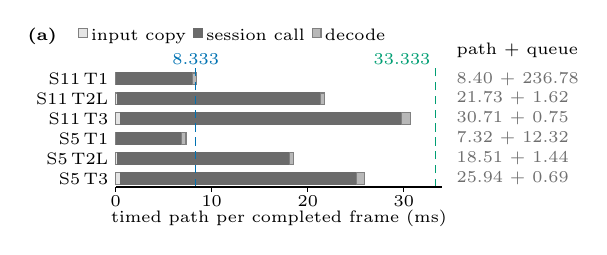
\begin{tikzpicture}[x=1pt,y=1pt,line width=0.4pt]
\definecolor{figblue}{RGB}{0,114,178}
\definecolor{figverm}{RGB}{213,94,0}
\definecolor{figgreen}{RGB}{0,158,115}
\definecolor{figgrey}{RGB}{110,110,110}
\providecommand{\fsix}{\fontsize{6}{7}\selectfont}
\draw[fill=black!10,draw=black!50] (32.00,79.00) rectangle (33.84,83.20);
\draw[fill=black!58,draw=black!58] (33.84,79.00) rectangle (118.94,83.20);
\draw[fill=black!28,draw=black!50] (118.94,79.00) rectangle (122.03,83.20);
\node[anchor=east,inner sep=0pt,font=\fsix] at (29.50,81.10) {S5\,T3};
\node[anchor=west,inner sep=0pt,font=\fsix,text=figgrey] at (155.00,81.10) {25.94 $+$ 0.69};
\draw[fill=black!10,draw=black!50] (32.00,86.20) rectangle (32.76,90.40);
\draw[fill=black!58,draw=black!58] (32.76,86.20) rectangle (94.89,90.40);
\draw[fill=black!28,draw=black!50] (94.89,86.20) rectangle (96.23,90.40);
\node[anchor=east,inner sep=0pt,font=\fsix] at (29.50,88.30) {S5\,T2L};
\node[anchor=west,inner sep=0pt,font=\fsix,text=figgrey] at (155.00,88.30) {18.51 $+$ 1.44};
\draw[fill=black!10,draw=black!50] (32.00,93.40) rectangle (32.42,97.60);
\draw[fill=black!58,draw=black!58] (32.42,93.40) rectangle (55.93,97.60);
\draw[fill=black!28,draw=black!50] (55.93,93.40) rectangle (57.42,97.60);
\node[anchor=east,inner sep=0pt,font=\fsix] at (29.50,95.50) {S5\,T1};
\node[anchor=west,inner sep=0pt,font=\fsix,text=figgrey] at (155.00,95.50) {7.32 $+$ 12.32};
\draw[fill=black!10,draw=black!50] (32.00,100.60) rectangle (33.82,104.80);
\draw[fill=black!58,draw=black!58] (33.82,100.60) rectangle (135.42,104.80);
\draw[fill=black!28,draw=black!50] (135.42,100.60) rectangle (138.57,104.80);
\node[anchor=east,inner sep=0pt,font=\fsix] at (29.50,102.70) {S11\,T3};
\node[anchor=west,inner sep=0pt,font=\fsix,text=figgrey] at (155.00,102.70) {30.71 $+$ 0.75};
\draw[fill=black!10,draw=black!50] (32.00,107.80) rectangle (32.65,112.00);
\draw[fill=black!58,draw=black!58] (32.65,107.80) rectangle (106.06,112.00);
\draw[fill=black!28,draw=black!50] (106.06,107.80) rectangle (107.43,112.00);
\node[anchor=east,inner sep=0pt,font=\fsix] at (29.50,109.90) {S11\,T2L};
\node[anchor=west,inner sep=0pt,font=\fsix,text=figgrey] at (155.00,109.90) {21.73 $+$ 1.62};
\draw[fill=black!10,draw=black!50] (32.00,115.00) rectangle (32.39,119.20);
\draw[fill=black!58,draw=black!58] (32.39,115.00) rectangle (59.63,119.20);
\draw[fill=black!28,draw=black!50] (59.63,115.00) rectangle (61.17,119.20);
\node[anchor=east,inner sep=0pt,font=\fsix] at (29.50,117.10) {S11\,T1};
\node[anchor=west,inner sep=0pt,font=\fsix,text=figgrey] at (155.00,117.10) {8.40 $+$ 236.78};
\draw[figblue,densely dashed] (60.92,78.00) -- (60.92,122.20);
\node[anchor=south,inner sep=1pt,font=\fsix,text=figblue] at (60.92,121.20) {8.333};
\draw[figgreen,densely dashed] (147.69,78.00) -- (147.69,122.20);
\node[anchor=south east,inner sep=1pt,font=\fsix,text=figgreen] at (146.89,121.20) {33.333};
\draw[draw=black] (32.00,78.00) -- (150.00,78.00);
\draw[draw=black] (32.00,78.00) -- (32.00,76.20);
\node[anchor=north,inner sep=1pt,font=\fsix] at (32.00,76.20) {0};
\draw[draw=black] (66.71,78.00) -- (66.71,76.20);
\node[anchor=north,inner sep=1pt,font=\fsix] at (66.71,76.20) {10};
\draw[draw=black] (101.41,78.00) -- (101.41,76.20);
\node[anchor=north,inner sep=1pt,font=\fsix] at (101.41,76.20) {20};
\draw[draw=black] (136.12,78.00) -- (136.12,76.20);
\node[anchor=north,inner sep=1pt,font=\fsix] at (136.12,76.20) {30};
\node[anchor=north,inner sep=0pt,font=\fsix] at (91.00,70.00) {timed path per completed frame (ms)};
\node[anchor=south west,inner sep=0pt,font=\fsix] at (155.00,124.70) {path $+$ queue};
\node[anchor=south west,inner sep=0pt,font=\fsix] at (0.0,129.20) {\textbf{(a)}

\
\ \tikz[baseline=-0.5ex]{\filldraw[fill=black!10,draw=black!50](0,0)rectangle(3.2pt,3.2pt);}\,input copy\ \tikz[baseline=-0.5ex]{\filldraw[fill=black!58,draw=black!58](0,0)rectangle(3.2pt,3.2pt);}\,session call\ \tikz[baseline=-0.5ex]{\filldraw[fill=black!28,draw=black!50](0,0)rectangle(3.2pt,3.2pt);}\,decode};
\end{tikzpicture}
}\hfill
\resizebox{0.475\textwidth}{!}{% Generated by tools/rbq_fig_*.py from committed records. Do not edit by
% hand: regenerate instead, so the figure and its manifest entry stay in
% step. Records read are listed in
% experiments/mmsys2027_rbq_retarget_20260914/paper_figures_20260915/FIGURES_R1.json.
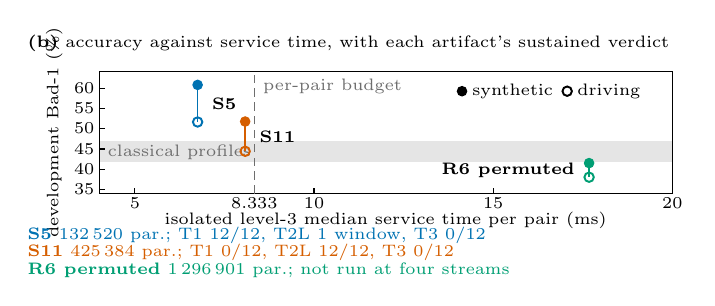
\begin{tikzpicture}[x=1pt,y=1pt,line width=0.4pt]
\definecolor{figblue}{RGB}{0,114,178}
\definecolor{figverm}{RGB}{213,94,0}
\definecolor{figgreen}{RGB}{0,158,115}
\definecolor{figgrey}{RGB}{110,110,110}
\providecommand{\fsix}{\fontsize{6}{7}\selectfont}
\fill[black!10] (26.00,11.27) rectangle (233.15,18.87);
\draw[draw=black] (26.00,0.00) rectangle (233.15,44.00);
\node[anchor=west,inner sep=1.5pt,font=\fsix,text=figgrey] at (27.50,15.07) {classical profiles};
\draw[draw=black] (26.00,1.47) -- (28.00,1.47);
\node[anchor=east,inner sep=1.5pt,font=\fsix] at (26.00,1.47) {35};
\draw[draw=black] (26.00,8.80) -- (28.00,8.80);
\node[anchor=east,inner sep=1.5pt,font=\fsix] at (26.00,8.80) {40};
\draw[draw=black] (26.00,16.13) -- (28.00,16.13);
\node[anchor=east,inner sep=1.5pt,font=\fsix] at (26.00,16.13) {45};
\draw[draw=black] (26.00,23.47) -- (28.00,23.47);
\node[anchor=east,inner sep=1.5pt,font=\fsix] at (26.00,23.47) {50};
\draw[draw=black] (26.00,30.80) -- (28.00,30.80);
\node[anchor=east,inner sep=1.5pt,font=\fsix] at (26.00,30.80) {55};
\draw[draw=black] (26.00,38.13) -- (28.00,38.13);
\node[anchor=east,inner sep=1.5pt,font=\fsix] at (26.00,38.13) {60};
\draw[draw=black] (38.95,0.00) -- (38.95,2.00);
\node[anchor=north,inner sep=1.5pt,font=\fsix] at (38.95,0.00) {5};
\draw[draw=black] (82.10,0.00) -- (82.10,2.00);
\node[anchor=north,inner sep=1.5pt,font=\fsix] at (82.10,0.00) {8.333};
\draw[draw=black] (103.68,0.00) -- (103.68,2.00);
\node[anchor=north,inner sep=1.5pt,font=\fsix] at (103.68,0.00) {10};
\draw[draw=black] (168.41,0.00) -- (168.41,2.00);
\node[anchor=north,inner sep=1.5pt,font=\fsix] at (168.41,0.00) {15};
\draw[draw=black] (233.15,0.00) -- (233.15,2.00);
\node[anchor=north,inner sep=1.5pt,font=\fsix] at (233.15,0.00) {20};
\draw[figgrey,densely dashed] (82.10,0.00) -- (82.10,44.00);
\node[anchor=north west,inner sep=1.5pt,font=\fsix,text=figgrey] at (83.60,43.00) {per-pair budget};
\node[anchor=north,inner sep=0pt,font=\fsix] at (129.57,-6.50) {isolated level-3 median service time per pair (ms)};
\node[rotate=90,anchor=south,inner sep=0pt,font=\fsix] at (13.00,22.00) {development Bad-1 (\%)};
\draw[figblue,line width=0.5pt] (61.61,39.28) -- (61.61,25.87);
\filldraw[fill=figblue,draw=figblue] (61.61,39.28) circle (1.7pt);
\draw[figblue,line width=0.7pt] (61.61,25.87) circle (1.7pt);
\node[anchor=west,inner sep=1.5pt,font=\fsix] at (65.11,32.58) {\textbf{S5}};
\draw[figverm,line width=0.5pt] (78.79,26.04) -- (78.79,15.29);
\filldraw[fill=figverm,draw=figverm] (78.79,26.04) circle (1.7pt);
\draw[figverm,line width=0.7pt] (78.79,15.29) circle (1.7pt);
\node[anchor=west,inner sep=1.5pt,font=\fsix] at (82.29,20.67) {\textbf{S11}};
\draw[figgreen,line width=0.5pt] (203.07,11.02) -- (203.07,5.92);
\filldraw[fill=figgreen,draw=figgreen] (203.07,11.02) circle (1.7pt);
\draw[figgreen,line width=0.7pt] (203.07,5.92) circle (1.7pt);
\node[anchor=east,inner sep=1.5pt,font=\fsix] at (199.57,8.47) {\textbf{R6 permuted}};
\node[anchor=west,inner sep=0pt,font=\fsix,text=figblue] at (0.0,-15.00) {\textbf{S5}\ 132\,520 par.; T1 12/12, T2L 1 window, T3 0/12};
\node[anchor=west,inner sep=0pt,font=\fsix,text=figverm] at (0.0,-21.40) {\textbf{S11}\ 425\,384 par.; T1 0/12, T2L 12/12, T3 0/12};
\node[anchor=west,inner sep=0pt,font=\fsix,text=figgreen] at (0.0,-27.80) {\textbf{R6 permuted}\ 1\,296\,901 par.; not run at four streams};
\filldraw[fill=black,draw=black] (157.15,37.00) circle (1.7pt);
\node[anchor=west,inner sep=2pt,font=\fsix] at (158.65,37.00) {synthetic};
\draw[black,line width=0.7pt] (195.15,37.00) circle (1.7pt);
\node[anchor=west,inner sep=2pt,font=\fsix] at (196.65,37.00) {driving};
\node[anchor=south west,inner sep=0pt,font=\fsix] at (0.0,51.00) {\textbf{(b)}\ accuracy against service time, with each artifact's sustained verdict};
\end{tikzpicture}
}
\caption{Camera-free replay of two artifacts under the three organizations at one offered load, four streams at 30 FPS each, and the plane they trace. (a) The timed per-frame path as pooled means, the queue wait printed rather than drawn because it is off scale at one organization; under T3 one call serves four frames sharing one path. Each condition pools 211,567 to 216,000 frames over three 600-s windows, except S5 under T2L, one window of 72,000. (b) Actual-accelerator development Bad-1 at level 3, macro over the 512-pair development population, against the isolated post-warmup median service time per pair; the band spans the four frozen classical profiles. No artifact reaches both axes.}
\label{fig:path}
\end{figure*}
One arm selected after its development numbers were seen bears on how a gate is read: the registered final 2,000-update stage moved its driving Bad-1 from 41.3807, passing both classical profiles in full precision, to the exported 42.3527, failing one by 0.53 points, while that earlier state is better on silicon at 43.0034 and still misses the three-path profile. A gate evaluated in full precision can be a property of that precision rather than of the artifact that reaches the device. That arm remains \emph{post-hoc selected}; in seeds 1 and 2 the same endpoint was pre-specified and also misses that profile on silicon. Building the joint organization on both artifacts is itself a result: a static batch-size-four rewrite of the 24- and 26-node graphs is refused by the backend at the same named layer with zero accelerator calls, separating the batch axis from the node count that confounded R6's refusal. A multi-input form---four identical copies with four input and four output ports in one call and no batch axis, at 96 and 104 nodes---places fully on both and passes the independence proof R6 failed: 200 repeat calls, three slot-order rotations and four changed-companion draws return zero differing elements, including the draw R6 failed at lane maxima of 68.4 against a range near $\pm$104. A four-pair call costs 0.90$\times$ four single calls on both, 24.308 against 27.000 ms and 29.219 against 32.308, neither the earlier line's 2.657$\times$ penalty nor a fourfold division. Both then fail the sustained joint protocol, and the two halves of the frozen rule separate. Every stream of every window rounds to 30.0 FPS and the completion floor is met, at 17,985 to 17,991 unique frames per stream on S11 and 17,991 to 17,994 on S5, yet every window carries replacements and the rule requires none (Table~\ref{tab:sustained}). Nothing failed numerically, across 215,856 and 215,904 timed 64-element probes. The mechanism is the period boundary: S11's timed path costs about 31.5 ms against 33.333, some 1.8 ms of slack, so a call in the upper tail of a 29.3-ms accelerator-call distribution overruns and the next period finds a slot empty. Raising the slack to about 6.6 ms on S5 halved the losses without removing them, because what overruns is the tail: S5's maxima reach 55.4 to 58.5 ms and 0.86 to 0.95\% of its frames pass one period, against 2.76 to 3.03\% on S11. That tail is not diagnosed.

Figure~\ref{fig:path}b places the three artifacts side by side; the organization decides every sustained verdict, S11 passing only under process isolation, S5 only under sequential serving and the joint organization for neither, buying a tenth of the per-call cost but not the tail.

\subsection{Four physical cameras of two models}
\label{sec:physical}
Every window above is camera-free replay. The study's physical runs feed S11, under the four-process organization that passed in replay, and then S5, from four physical stereo cameras of two models: three OAK-D-W Pro units and one Intel RealSense D435i. \emph{The mix was not a design choice}: the rig's fourth OAK rebooted about every 13~s on three different USB root controllers, and the heterogeneous set was registered as a separate experiment before any window, so it is never counted as the registered all-OAK run, which was then not performed by decision. Each OAK stream is that device's rectified $1280\times800$ mono pair; the RealSense stream is its two infrared imagers, delivered rectified at $1280\times720$ with the projector off, which the producer confirms from all-zero distortion coefficients before it publishes. One frozen resize maps both to the $416\times256$ tier, squeezing the RealSense picture more anisotropically; no accuracy is measured, so that difference is recorded rather than scored.

S11 passed, and S5 then passed from the same cameras under its own passing organization (Table~\ref{tab:sustained}, last two rows): three 600-s windows each, 17,998 to 18,000 unique frames against the floor of 17,970, zero replacements, strict NPU-only placement in every session, and every integrity comparison exact, including 48 live frames per window re-run after it and a cross-check against an earlier independent capture of each artifact. Two caveats travel with those verdicts. The harness's own unrounded flag, which the replay windows met at exactly 18,000, reads fail in all six, because free-running camera clocks delivered one or two frames fewer in ten minutes; the registered rule rounds. And the response is not the replay's: timed from the capture stamp, about 55~ms at the median is the path before the accelerator---device rectification and pair sync, USB transport and the host resize---while the accelerator-side work averages 13.3 to 13.8~ms for S11 under four sessions and 6.8 to 9.0~ms for S5 under one. \emph{Measured from the OAK exposure end, no completed OAK frame arrives within one 33.333-ms period}, in any of the eighteen OAK stream-windows. The RealSense stream's lower figures are not evidence of a faster camera: it stamps a frame timestamp of a different meaning, declared before the run, so the two models' responses are not compared.

Reaching S11's verdict took four attempts of the registered six-run budget, and what failed describes this host. Its control temperature reached 95~$^\circ$C within seconds of any CPU burst while the board sensors stayed near 50~$^\circ$C, aborting runs in turn during compilation, at the start of inference where camera start-up and session initialization coincided, and before start. Each repair moved an ordering, never a threshold: the inference-phase rule never changed, and under it the passing windows peaked at 82.4~$^\circ$C. The last repair has a price, since running the cameras through compilation raised its peak from at most 72.0 to 99.5--100.0~$^\circ$C, and two runs of the eight across both artifacts hit the retained 100~$^\circ$C ceiling and were voided. Earlier attempts contributed two further passing windows, not counted here; no window that completed ever failed.

The run also exposed a latent defect in the all-OAK capture path, which requests a colour image type from a mono sensor: 23.46~FPS with 39 of 180 frames dropped on the device, against 30.00~FPS and none for the native grayscale type, whose rectified bytes are identical in 30 of 30 sequence-matched captures. The request itself succeeds and every earlier window used a synthetic producer, so replay could not have shown it.

\section{Limitations and Conclusion}
A four-stream operating point exists: the common model's process-isolated pair organization and its one-session joint organization each completed three 600-s repetitions at the target rate with exact outputs and zero CPU neural nodes, while six streams screened out---the limit reached by the layouts screened here, not of stereo matching. One stream passed and two were integrity-negative in both organizations, so integrity did not follow the stream count. Its endpoint error improves on the device default in every scene of both benchmark sets at $p_{\mathrm{holm}} = 3.81\times10^{-6}$, while no bad3 advantage is claimed. Both speed-line artifacts, each in its own passing organization, also sustained that protocol from four physical cameras of two models---the study's only physical runs---though no OAK frame completed within one period of its exposure. None of the eight specialized candidates passed after fixed 8-bit export and the recovered development survivor stopped at its first raw-output check in all three board configurations, while a value-preserving rewrite recovered 98.0\% of one artifact's block floating-point deployment loss without retraining---an artifact that still misses the device-default comparator on one of four comparisons, its full-precision source more widely, and on which two preregistered geometric repairs failed out of sample.

Limitations constrain every claim. No accuracy was measured in the 0.15--0.5 m near range the robot's step specification implies, and no calibrated distance target was available, so disparity error here is not distance error. All runtime results but two are camera-free replay, and those two used a heterogeneous camera set, one organization per artifact, measured no synchronization and served no OAK frame within one period of its exposure; no all-OAK physical run was performed, and cross-device synchronization and any claim about per-frame latency from capture are untested; accuracy evidence is development-only, both sealed sets unopened and the second campaign's four mandatory secondary reports never evaluated; the common model carries a shared pretrained parent and uncertain teacher lineage. The raw-output mismatch cause is unresolved, the literal oracle is qualification instrumentation rather than an online detector, and its in-window probe samples 64 elements. The speed-first line adds its own: one seed for S5 and three for S11, whose two extra seeds were authorized by waiver after the seed-0 accelerator audit failed, and confirmation seeds never started; selection-exposed development figures for both trained artifacts; one process-isolated window behind S5's tail claim against three for S11; no published matcher was compiled on this device, so the placement refusals and service times are properties of these graphs; a deadline-miss share of about a fifth of frames in the passing process-isolated windows, which the throughput protocol does not test; the undiagnosed joint-call tail; and one post-hoc arm. All measurements come from one installation with unchanged driver and firmware, the second campaign pairing a vendor userspace with an older host driver in a combination its records mark unverified; package energy includes host activity, physical partitioning was not demonstrated, and seed confirmations and a final evaluation are outstanding.


\section*{Generative AI Disclosure}
Generative AI assisted the drafting, the figures, the tables and the evaluation code and analysis;
the authors are responsible for all content.
\bibliographystyle{ACM-Reference-Format}
\bibliography{references}%, references_rbq_additions}
\end{document}
